\documentclass[a4paper]{article}

%% Language and font encodings
\usepackage[english]{babel}
\usepackage[utf8x]{inputenc}
\usepackage[T1]{fontenc}
\usepackage{algpseudocode} 
\usepackage{float}
\usepackage{booktabs}
%% Sets page size and margins
\usepackage[a4paper,top=3cm,bottom=2cm,left=3cm,right=3cm,marginparwidth=1.75cm]{geometry}

%% Useful packages
\usepackage{amsmath}
\usepackage{graphicx}
\usepackage{qtree}
\usepackage[colorinlistoftodos]{todonotes}
\usepackage[colorlinks=true, allcolors=blue]{hyperref}
\usepackage{tikz}
\usetikzlibrary{automata,positioning}

\usepackage{forest}
\renewcommand{\rmdefault}{ptm}

\begin{document}
\section*{RANGE UPDATES}
Consider an array C of n integers, initially all equal to zero. We want to support the following operations:
\begin{itemize}
\item update(i, j, c), where 0 $\leq i \leq j \leq n \leq 1$ and c is an integer: it changes C such
that $C[k] := C[k] + c$ for every $i \leq k \leq j$.
\item query(i), where $0 \leq i \leq n \leq 1$: it returns the values of$ C[i]$.
\item sum(i, j), where $0 \leq i \leq j \leq n \leq 1$: it returns $\sum_{k=i}^{j} C[k]$
\end{itemize}
Design a data structure that uses O(n) space and implements each operation above in O(log n) time. Note that query(i) = sum(i, i) but it helps to reason. [Hint to further save space: use an implicit tree such as the Fenwick tree (see Wikipedia).]\\
\\
\textbf{SOLUTION WITH RANGE TREE}
\\
Given the problem, in which we want to efficiently (log. time, and linear
space) work with values stored in an array contained within an arbitrary
range \([1...n]\), we need to implement:

\begin{itemize}
\item
  Updating a portion of the range by adding a value c: Update(i, j, c).
\item
  Querrying the value on a given index: Query(i).
\item
  Obtaining the sum of all elements within a range: Sum(i, j).
\end{itemize}

A possible solution is to model the range as trees, with branches
partitioning the overall ranges in smaller ones to efficiently operate
on them. Leaves store discrete indices while their parents represent the
index ranges contained under them. A tree for \(n=8\), with indices
\([0...7]\) is shown below:

\begin{figure}[htbp]
\centering
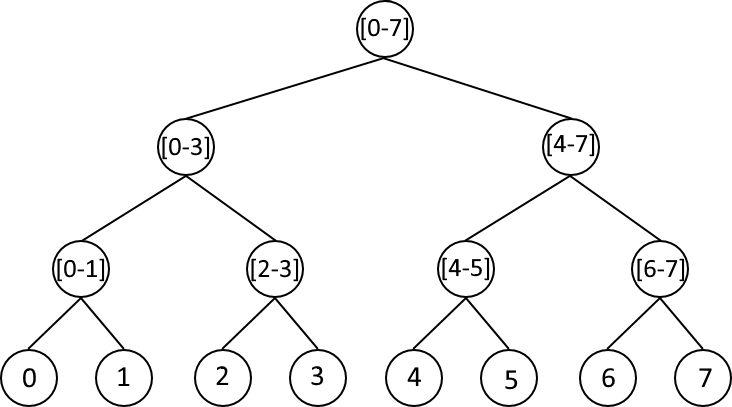
\includegraphics[scale=0.45]{Tree.png}
\caption{Tree for N=8}
\end{figure}
Space-wise, this means that for an array of length \(n\), we will at
most require \(\sum\limits_{i=0}^{\infty} \frac{n}{2^i}\) nodes in the
tree, as \(\frac{n}{2}\) parents will be needed for the n leaves,
\(\frac{n}{4}\) for those parents and so on. This geometric series
converges to \(2n\), leaving us a space complexity bound of \(O(n)\).\\
The implementation of 1-value query is simple: we use the intervals
to binary-search our target node. In doing so, we traverse only one tree
branch, with time complexity \(O(log\ n)\).\\
Updating and range-summing, on the other hand, are trickier. For them to
be efficient, we need to process a whole interval in \(O(log\ n)\).
To do so, we perform the same binary-search process as before, stopping
when the current interval matches the interval of the node. Otherwise we further splitting the interval towards their sub-trees.
On a given tree, such splitting will happen at most on \(log(n)- 1\)
times on both interval extreme, when the range covers all but there is an extreme of the
interval that is not fully included. When the intervals match, the marking operation will be applied.
\\
Finally, to efficiently implement both range operations, branch nodes
that represent intervals will require two variables: the amount that is
added in common to all of their successors and the total sum of their
values. That way, operations onto a given node will remain \(O(1)\),
with our previous analysis being applicable translating into a time
complexity bounded by \(O(log\ n)\).
\newpage \qquad \\
\textbf{SOLUTION WITH BIT TREE}
\\
The solution can be implemented using a Segment tree or a Fenwick Tree. Both allowed the aforementioned operation in O(log n). Here we will present a solution that use Fenwick Trees also called Binary Indexed Tree (BIT).\\
Let's start with some considerations: 
\begin{itemize}
\item integer can be represented as sum of powers of two. Therefore, I can represent the sum operation as sum of sets of sub-sums.
\item each index, if it is a power of 2, will store the sum of all elements before that, and we will apply this repetitively so as to get what each index will store. Let's see an example:
\\ 
Suppose, we have an array of 16 elements, $[1 \dots 16]$. Powers of 2 are the index: 1, 2, 4, 8, 16. These index will store sum of all elements before them. Now, we divide this array in two halves: we get $[1 \dots 8]$ and $[9 \dots 16]$, and so on. \\
Let's have the following array: 
\begin{align}
\nonumber
A  &=[1,2,3,4,5,6,7,8]\\
BIT&=[0,0,0,0,0,0,0,0]
\end{align}

Let take the power 2 index (i.e. 1,2,4,8), and we store in BIT the value of the sum of the previous element. Then we have:
\begin{align}
\nonumber
BIT=[1,3,0,10,0,0,0,36]
\end{align}

Now we divide the array in two: $A_1=[1,2,3,4]$ and $A_2=[5,6,7,8]$. Then we take the power 2 index of $A_1$ and $A_2$ (i.e. 1,2,4), and we update the value of BIT where there index that are not updated yet. Then we have:
\begin{align}
\nonumber
BIT=[1,3,0,10,5,11,0,36]
\end{align}

Following the same procedure, the value doesn't change at any index if it has been already filled. Then we will the following. 
\begin{align}
\nonumber
BIT=[1,3,3,10,5,11,7,36]
\end{align}
If we consider our array as a binary tree, and we change the value of each node by adding the sum of nodes in its left sub-tree, we will obtain the same result.
\item Now let's see how to implement sum(i, j). The idea is to keep a variable $ans$ initialized to 0. Follow the path from $root$ to the $index$ node. Whenever we need to follow a right link, add the value of current node to $ans$, and once we reach the node with the searched index we add that value too. To get the sum of elements in range i to j,  we get the sum from 0 to j and we subtract the sum from 0 to (i-1). 
\item Now let's see how to implement update(i, j, c). For now we focus on just the update of a single index. If we want to increment the value at index $k$ by say $c$. Follow the path from root to the index node $k$. Whenever we need to follow a left link, add the value of $c$ to current node. Once we reach the node, add $c$ to that node too. This is because we will need to update the set of nodes in the tree that include that node in its left sub-tree, so that it will be consistent with our sum operation.
\end{itemize}
\qquad \\
\iffalse
Let's start by converting all the index in binary. For each index, find the right most SET-bit (i.e. '1') and drop all zeros on its right and side along with the considered '1'. For example:
\begin{align}
\nonumber
100 & \longrightarrow empty\\
101 & \longrightarrow 10\\
111 & \longrightarrow 11\\
010 & \longrightarrow 0\\
\end{align}
Here is the thing to be observed. If we treat 0 as LEFT and 1 as RIGHT, each node tells you the path to be followed from root to reach that node. For example we have:\\
\\
\\
\Tree [.4 [.2 1 3 ] [.6 5 7 ] ] 
\Tree [.100 [.010 001 011 ] [.110 101 111 ] ] 
\Tree [.- [.0 00 01 ] [.1 10 11 ] ] 
\\
\fi 
To implement this kind of idea we need to exploit some properties of the binary numbers. Since for the sum function we need the right-path we exploit the following fact: given an index if we reset the right-most SET-bit we will go up to the least node that took a RIGHT path. For example:
\begin{align*}
&\Tree [.4 [.2 1 3 ] [.6 5 7 ] ] \qquad \qquad \qquad\qquad
\Tree [.100 [.010 001 011 ] [.110 101 111 ] ] \\ 
5 &\longrightarrow 101 \longrightarrow 100 \longrightarrow 4 \\
7 &\longrightarrow 111 \longrightarrow 110 (6) \longrightarrow 100 \longrightarrow 4 \\
3 &\longrightarrow 011 \longrightarrow 010 \longrightarrow 2\\
\end{align*}
To implement this concept in to an algorithm we use the following formula $i - (i \ AND (-i))$, where $i$ is the current index and $(-i)$ mean the 2's complement of $i$.
\begin{algorithmic}
\Function{getSum}{$index$} 
\State $ans\gets 0$
\While{$index \ > 0$} 
	\State $ans \gets ans +BIT[index]$
	\State $index \gets index - (index \ AND (-index))$	
\EndWhile
\State \Return $ans$
\EndFunction
\end{algorithmic}
Now we should try to do the same for the updating function. Now given an index we should search the least node that took the LEFT path. Here, instead of stripping off the least-significant 1 bit (i.e. subtracting), we now add it on at each stage to get the next entry to adjust. Therefore we simply have:
\begin{algorithmic}
\Function{update}{$index$,$val$} 
\While{$index \ < length\_of\_array$} 
	\State $BIT[index] \gets BIT[index] +val$
	\State $index \gets index + (index \ AND (-index))$	
\EndWhile
\State \Return $ans$
\EndFunction
\end{algorithmic}
\qquad \\
\\
\\
Notice that getSum and update work in O(log n), where n is the length of the input. However, the update function modify one element at the time, then we still need to find a way to do a range update in O(log n). The idea is to keep two BIT (i.e. BIT1 and BIT2) and then modify the functions to sum and update a range. \\
\\
Let's start with the update function update(i, j, c). When we update BIT1 we will use the previous update as follow:
\begin{align*}
update(i, c)  \qquad & \# \textit{in BT1}\\ 	
update(j + 1, -c)  \qquad & \# \textit{in BT1}
\end{align*}
The idea is that the $update(i, c)$ will affect all $i' \leq i$, i.e all the left subtree where we store the partial sum of the sub-interval. To limit the effect to a given range $[i,...,j]$, we subtract $-c$ from all $i' > j$ by performing the operation $update(j+1, -c)$. Now, if we use the getSum function as it is, we will have a wrong result. Indeed we should find a way to tell how much the results have to be adjust, here comes the second BIT (i.e BT2). 
Consider a range $update(i,j,c)$ and let all the elements at the beginning were 0. Now, let consider a getSum(p) for a generic $p$, then we have:
\begin{align*}
1 & \leq p < i \longrightarrow 0 \\
i & \leq p \leq j \longrightarrow c*(p-(i-1))\\
j & < p \leq N \longrightarrow c*(j-(i-1))
\end{align*}
Thus, for a given index $p$, expanding those formula we obtain the term needed to adjust the prefixed sum. Indeed we find a term $X$ in this way:
\begin{align*}
1 & \leq p < i \longrightarrow 0 \longrightarrow X=0\\
i & \leq p \leq j \longrightarrow c*p - c*(i-1)\longrightarrow X= c*(i-1) \\
j & < p \leq N \longrightarrow c*j - c*(i-1) \longrightarrow X= -c*j + c*(i-1)
\end{align*}
This extra factor keep track of the adjustment needed to obtain the correct sum. To maintain this extra factor $X$, we use another BIT(i.e BT2) then we have:
\begin{align*}
update(i, c * (i-1))     \qquad     &\#\textit{in BT2} 	\\
update(j + 1, -c * j) 	\qquad	&\#\textit{in BT2}
\end{align*}
Notice $c*(i-1)$ it's not there because it has been included in the previous update. Indeed to obtain a correct range sum we have to do the following:
\begin{align*}
getSum(p)= getSum(BIT1,p) *p - getSum(BIT2,p)
\end{align*}
Finally we have the function requested in the exercise:
\begin{itemize}
\item $update(i, j, c)$ is equivalent to the following function:
\begin{itemize}
\item $update(BIT1,i, c)$
\item $update(BIT1,j + 1, -c)$
\item $update(BIT2,i, c * (i-1))$
\item $update(BIT2,j + 1, -c * j)$
\end{itemize} 
\item $query(i)= getSum(i)-getSum(i-1)$
\item $sum(i, j)=getSum(j)-getSum(i-1)$
\end{itemize} 
Both sum, query and update work in O(4 log(n)). This because: the tree is always balanced and the two function they simply take a path in the tree. Furthermore, this algorithm take just O(2 n) space since it's just storing a flat array.\footnote{Some references: 
\href{https://www.cs.auckland.ac.nz/~peter-f/FTPfiles/TechRep88.pdf}{LINK1}, 
\href{https://www.hackerearth.com/practice/notes/binary-indexed-tree-made-easy-2/}{LINK2},
\href{https://kartikkukreja.wordpress.com/2013/12/02/range-updates-with-bit-fenwick-tree/}{LINK3},
\href{http://stackoverflow.com/questions/27875691/need-a-clear-explanation-of-range-updates-and-range-queries-binary-indexed-tree/27877427\#27877427}{LINK4} and 
\href{http://cs.stackexchange.com/questions/33014/range-update-range-query-with-binary-indexed-trees}{LINK5}}
\end{document}